\section{Introduction to Crowd Counting}

\begin{frame}
\frametitle{Crowd Counting}

\begin{itemize}
\item Given a crowd image $\boldsymbol{X} \in \mathbb{R}^{H \times W \times C}$, \textbf{crowd counting} aims to automatically calculate the size $c$ of the crowd.
\item The ground truths in SOTA datasets \footnote{For example, ShanghaiTech A \& B \cite{zhang2016single}, UCF-QNRF \cite{idrees2018composition} and NWPU-Crowd \cite{wang2020nwpu}.} are density maps $\boldsymbol{Y} \in \mathbb{R}^{H \times W}$ instead, with
$$
\boldsymbol{Y}_{i, \, j} =
\begin{cases}
    1 & \quad \text{$\boldsymbol{X}_{i, \, j, \, :}$ denotes a person} \\
    0 & \quad \text{otherwise}
\end{cases}
$$
Thus, $c = \sum_{i=1}^H \sum_{j=1}^W |\boldsymbol{Y}_{i, \, j}|$.
\end{itemize}

\begin{center}
\begin{tikzpicture}
    \draw (2, 0) -- (2, 1) -- (2, 2);
    \draw (3, 0) -- (3, 1) -- (3, 2);
    \draw (4, 0) -- (4, 1) -- (4, 2);
    \draw (5, 0) -- (5, 1) -- (5, 2);
    \draw (2, 0) -- (3, 0) -- (4, 0) -- (5, 0);
    \draw (2, 1) -- (3, 1) -- (4, 1) -- (5, 1);
    \draw (2, 2) -- (3, 2) -- (4, 2) -- (5, 2);
    \node[anchor=center] at (2.5, 0.5) {\Smiley[2]};
    \node[anchor=center] at (3.5, 0.5) {\Moai[2]};
    \node[anchor=center] at (4.5, 0.5) {\Ninja[2][violet]};
    \node[anchor=center] at (2.5, 1.5) {\Cat[2]};
    \node[anchor=center] at (3.5, 1.5) {\Strichmaxerl[2]};
    \node[anchor=center] at (4.5, 1.5) {\Summertree[2]};
    \draw [-stealth] (5.5, 1) -- (6.5, 1);
    \node[anchor=west] at (7, 1) {$\begin{bmatrix} 0 & 1 & 0 \\ 1 & 0 & 1\end{bmatrix}$};
\end{tikzpicture}
\end{center}
\end{frame}

\begin{frame}
\frametitle{Crowd Counting}

\begin{figure}[htbp]
\centering
\begin{minipage}{.45\textwidth}
\centering
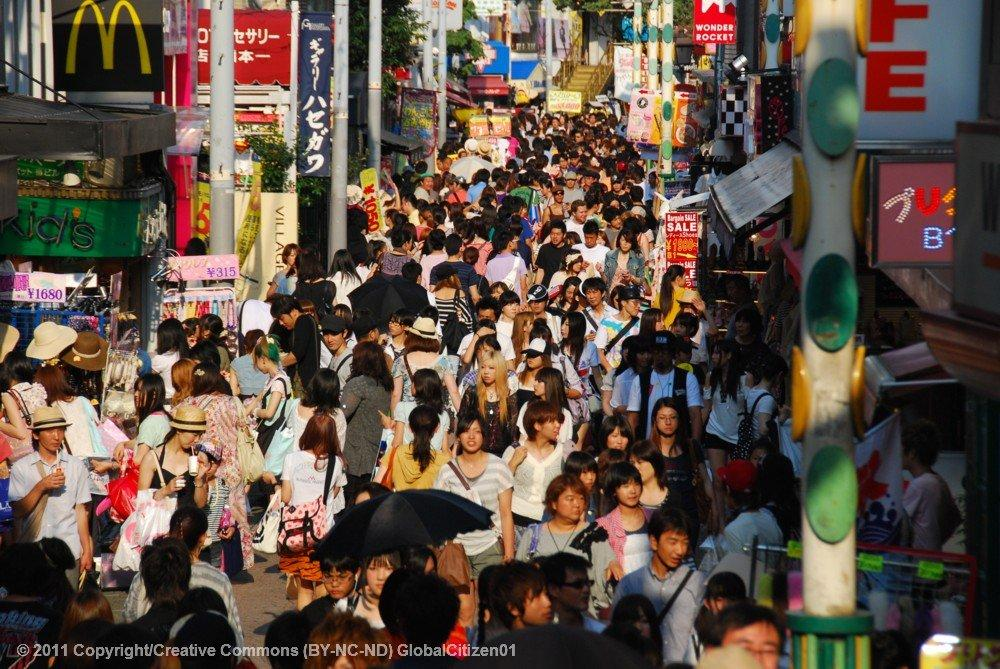
\includegraphics[width=0.95\linewidth]{images/img.jpg}
\end{minipage}%
\begin{minipage}{.45\textwidth}
\centering
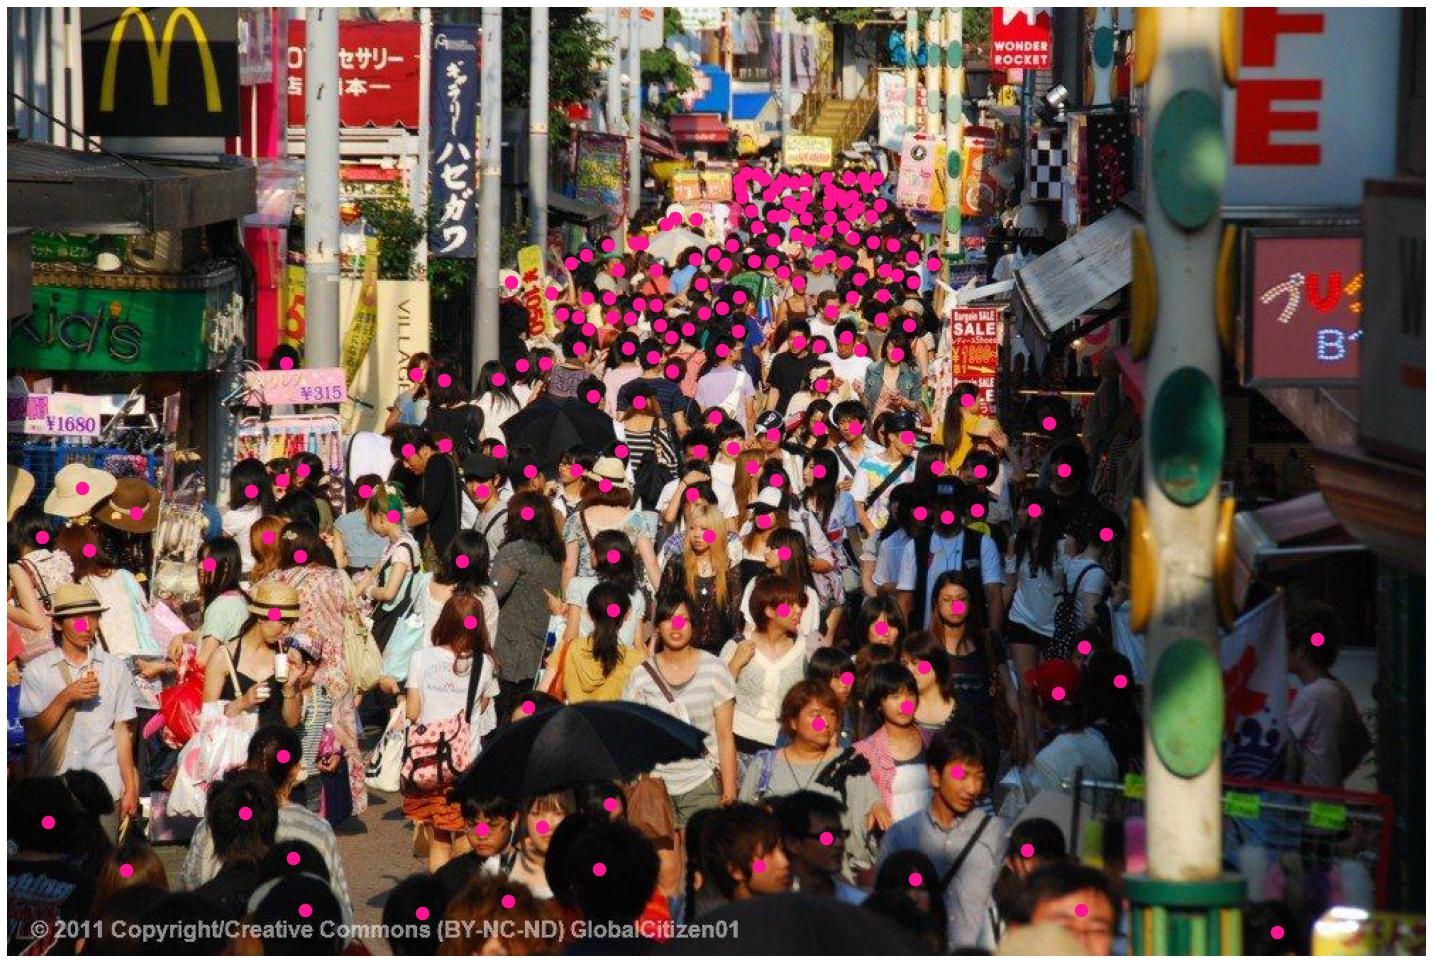
\includegraphics[width=0.95\linewidth]{images/img_with_ann.jpg}
\end{minipage}
\label{fig:1}
\caption{a crowd image and its annotations.}
\end{figure}

\end{frame}
